\section{Clamped Planform Loft, Bound Sensitivity and Mass Balance}
\label{sec:geometric_manifold}

\subsection{Planform Loft and Chord Clamp}
\label{sec:loft_def}
The planform is built from the design vector as follows (Fig.~\ref{fig:geometric_manifold}). Over the center body, $y \in [0, y_b]$ with $\xi = y/y_b$ and $t_\Lambda = \tan\Lambda_{\mathrm{in}}$, the leading edge is a cubic with zero slope at the symmetry plane and the trailing edge is a straight line from the root trailing edge to the blend-station trailing edge:
\begin{equation}
x_{\mathrm{LE}}(y) = t_\Lambda\, y_b\,\big(2\xi^2 - \xi^3\big), \qquad x_{\mathrm{TE}}(y) = c_r + \big(t_\Lambda\, y_b + c_b - c_r\big)\,\xi .
\label{eq:le_te}
\end{equation}
The chord is their difference,
\begin{equation}
c(y) = c_r + y_b\,\big[\, t_\Lambda\,\xi\,(1-\xi)^2 - \delta\,\xi \,\big], \qquad \delta = \frac{c_r - c_b}{y_b},
\label{eq:chord_cb}
\end{equation}
which equals $c_r$ at the root and $c_b$ at the blend station. Outboard of the blend station the leading edge is straight with sweep $\Lambda_{\mathrm{out}}$ and the chord tapers linearly from $c_b$ to $c_t = \lambda c_b$. The leading edge is therefore smooth at the symmetry plane and continuous, with a change of sweep, at the blend station. Twist varies linearly from $\theta_0$ to $\theta_1$ over the center body and piecewise linearly through $\theta_2$ (mid outer wing) to $\theta_t$ at the tip. The section is the MH91 reflexed airfoil at the root (maximum thickness $15.0\%$ of chord), blended linearly into the MH60 airfoil ($10.1\%$) at the blend station and kept constant outboard.

\begin{figure}[htbp]
\centering
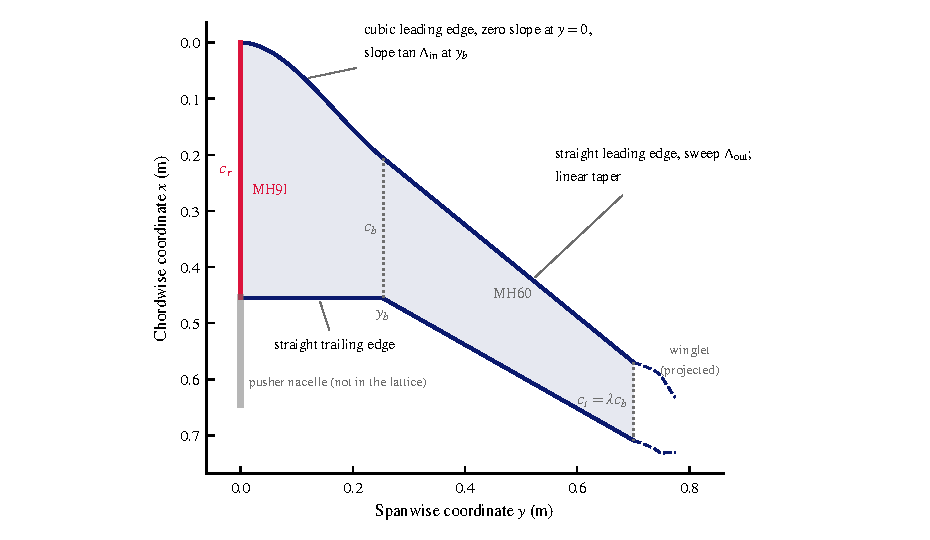
\includegraphics[width=\linewidth]{figures/figure2_geometric_manifold.pdf}
\caption{Planform parameterization: inner and outer leading-edge sweep $\Lambda_{\mathrm{in}}, \Lambda_{\mathrm{out}}$, blend station $y_{b}$, station chords $c_{r}, c_{b}, c_{t}$, the airfoil transition from MH91 to MH60 over the center body, and the pusher nacelle.}
\label{fig:geometric_manifold}
\end{figure}

\paragraph{Clamp} Before lofting, the builder clips the station chords so that they are ordered with a margin of $0.05\,\mathrm{m}$:
\begin{equation}
c_b \leftarrow \min\!\big(\max(c_b,\, 0.25),\; c_r - 0.05\big), \qquad c_t \leftarrow \min\!\big(\max(\lambda c_b,\, 0.05),\; c_b - 0.05\big).
\label{eq:clamp}
\end{equation}
This clamp is what the preprint of this work called a geometric manifold. It guarantees $c_r > c_b > c_t$, so the blend-station chord can never exceed the root chord, and the linear outer taper is monotone.

\paragraph{What the clamp does not guarantee} The clamp orders the three station chords; it does not make the chord monotone between the root and the blend station. Differentiating Eq.~\eqref{eq:chord_cb},
\begin{equation}
\frac{dc}{dy} = t_\Lambda\,(1-\xi)(1-3\xi) - \delta ,
\end{equation}
which is largest at the symmetry plane, where it equals $t_\Lambda - \delta$. The chord is therefore non-increasing over the whole center body if and only if
\begin{equation}
\tan\Lambda_{\mathrm{in}} \;\le\; \frac{c_r - c_b}{y_b},
\label{eq:mono}
\end{equation}
a condition that neither the clamp nor the bounds impose. When it is violated the chord first grows slightly outboard of the root before decreasing. Over the \NvMonoN\ valid designs of the original campaign, \NvMonoViolShare\% violate Eq.~\eqref{eq:mono}; the local growth of the chord has a median of \NvMonoMedian\,mm among them, exceeds $1\,\mathrm{mm}$ in \NvMonoGtOne\% of all valid designs and is at most \NvMonoMax\,mm (about $1\%$ of the root chord). The effect is small, but an earlier version of this manuscript stated a proof of spanwise chord monotonicity; that proof applied to a smoothstep chord law that the bay-volume estimate uses, not to the loft of Eq.~\eqref{eq:le_te} that the aerodynamic model uses, and it is withdrawn.

\subsection{Clamp Activity and Controlled Benchmark}
\label{sec:loft}
A preliminary study of $1{,}000$ Latin hypercube designs with uncoupled chord bounds (Supplementary Section~\ref{sec:ablation_study}) found a lower maximum $L/D$ among chord-inverted planforms, but the difference disappears when the designs are matched by reference area ($p = 0.49$), so that sample gives no evidence that chord inversion by itself lowers the efficiency computed by this pipeline. The controlled test is the following.

Within the bounds of the optimization ($c_{b} \in [0.25, 0.35]\,\mathrm{m}$, $c_{r} \in [0.42, 0.52]\,\mathrm{m}$, $\lambda \ge 0.55$) the clamp of Eq.~\eqref{eq:clamp} can never change a design: the largest blend chord is $0.07\,\mathrm{m}$ below the smallest root chord, and the taper floor keeps the tip chord above $0.05\,\mathrm{m}$ and more than $0.05\,\mathrm{m}$ below the blend chord. In a ten-seed search inside these bounds the clamp condition was met in none of the 2,870 evaluations. The designs reported in this paper were therefore not shaped by the clamp.

\begin{figure}[htbp]
\centering
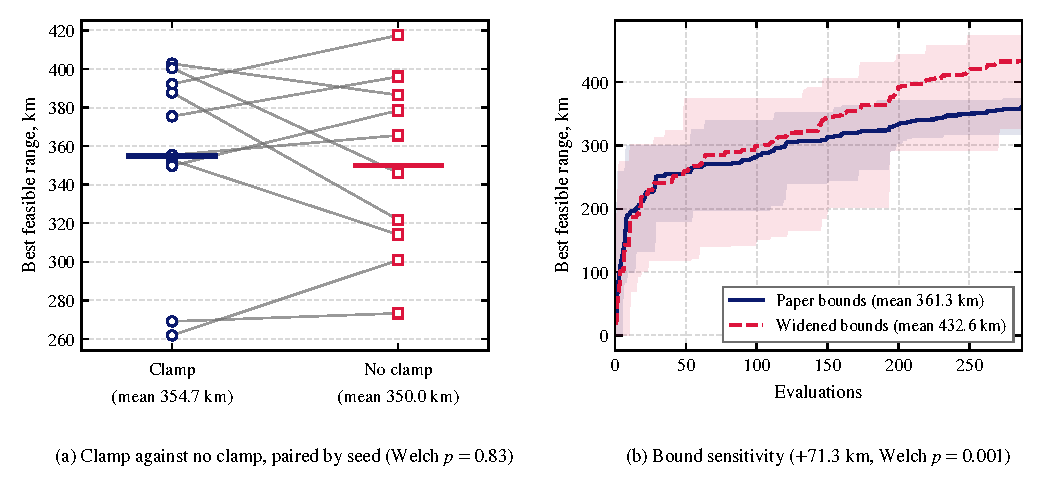
\includegraphics[width=\linewidth]{figures/fig_manifold_bounds.pdf}
\caption{Controlled loft and bound experiments, ten seeds each, 287 evaluations, no pool. (a) Best range of each seed with and without the chord clamp, blend-chord bound widened to $c_b \in [0.15, 0.65]\,\mathrm{m}$; lines join runs with the same seed and bars mark the means. (b) Mean running best with the original bounds and with four bounds relaxed; bands are the minimum-to-maximum envelopes over seeds.}
\label{fig:manifold_bounds}
\end{figure}

To test whether the clamp helps when the bounds do permit inversion, a controlled ten-seed experiment was run with the blend-chord bound widened to $c_{b} \in [0.15, 0.65]\,\mathrm{m}$. Both arms use the same search (48 Latin hypercube designs followed by Gaussian perturbations of the ten best designs found so far, 287 evaluations in total, no pool), the same seeds and the production evaluator; the only difference is that the two clipping lines of Eq.~\eqref{eq:clamp} are removed in the second arm. As presented in Table~\ref{tab:loft} and Fig.~\ref{fig:manifold_bounds}(a), the clamped search achieved a mean range of \NclampMean\,km compared to \NnoclampMean\,km for the unconstrained search ($\Delta = +4.7\,\mathrm{km}$, $p = 0.83$ via Welch's $t$-test and $p = 0.70$ via paired seed test). The clamped search was better in 4 of the 10 paired seeds, and the 95\% interval of the paired difference is about $[-22, +31]\,\mathrm{km}$, so effects of up to about $8\%$ in either direction cannot be excluded by this test.

The evidence therefore supports a limited statement. The clamp is a validity guard on the ordering of the station chords: it is never triggered inside the bounds used for the optimization, and when the bounds are widened until it is triggered in most samples it shows no measurable effect on the best range found. No claim is made that it improves the optimization.

\subsection{Exploration Bound Sensitivity Analysis}
\label{sec:bound_sensitivity}
To measure how much the result depends on the bounds, the same ten-seed search was run inside the bounds of Table~\ref{tab:design_bounds} and with four bounds relaxed, namely those on which the best designs of the original campaign lie: the battery-mass cap ($3.5 \to 4.5\,\mathrm{kg}$), the taper-ratio floor ($0.55 \to 0.35$), the winglet-twist cap ($0^\circ \to +5^\circ$) and the blend-chord cap ($0.35 \to 0.45\,\mathrm{m}$). The cruise-speed floor is a mission requirement and was not relaxed.

As reported in Table~\ref{tab:loft} and Fig.~\ref{fig:manifold_bounds}(b), relaxing the exploration bounds increased the mean discovered operational range from \NpaperBndMean\,km to \NwideBndMean\,km, a gain of $71.3$\,km ($+19.7\%$, Welch $p = 0.001$), with the best run reaching \NwideBndMax\,km. These runs use a simple elite search without the pool, so their absolute values are not comparable with Table~\ref{tab:budget}; only the difference between the two arms is interpreted.

The best designs are thus limited by the bounds and are not interior optima; no global optimality is claimed. Table~\ref{tab:bound} shows on which bounds the twenty best designs of the original database lie, and Section~\ref{sec:bound_prices} measures the range cost of the individual bounds, of which only the battery-mass cap turns out to be measurable.

\subsection{Mass and Center-of-Gravity Build-Up and Trim Constraints}
\label{sec:dynamic_balance}
Longitudinal equilibrium for a tailless aircraft requires satisfying the moment equation~\cite{nelson1998flight}:
\begin{equation}
C_m(\alpha) = C_{m0} + \left(\frac{x_{\mathrm{cg}} - x_{\mathrm{np}}}{\bar{c}}\right) C_L(\alpha)
\end{equation}
To achieve trimmed flight ($C_m = 0$) at cruise lift $C_{L,\mathrm{cruise}}$ without deploying elevon control surfaces, the planform must generate a positive zero-lift pitching moment:
\begin{equation}
C_{m0} = SM \cdot C_{L,\mathrm{cruise}} > 0
\label{eq:trim_req}
\end{equation}
This positive moment is synthesized through reflexed airfoil camber combined with negative wingtip twist ($\theta_t \in [-12^\circ, -2^\circ]$).

\begin{figure}[htbp]
\centering
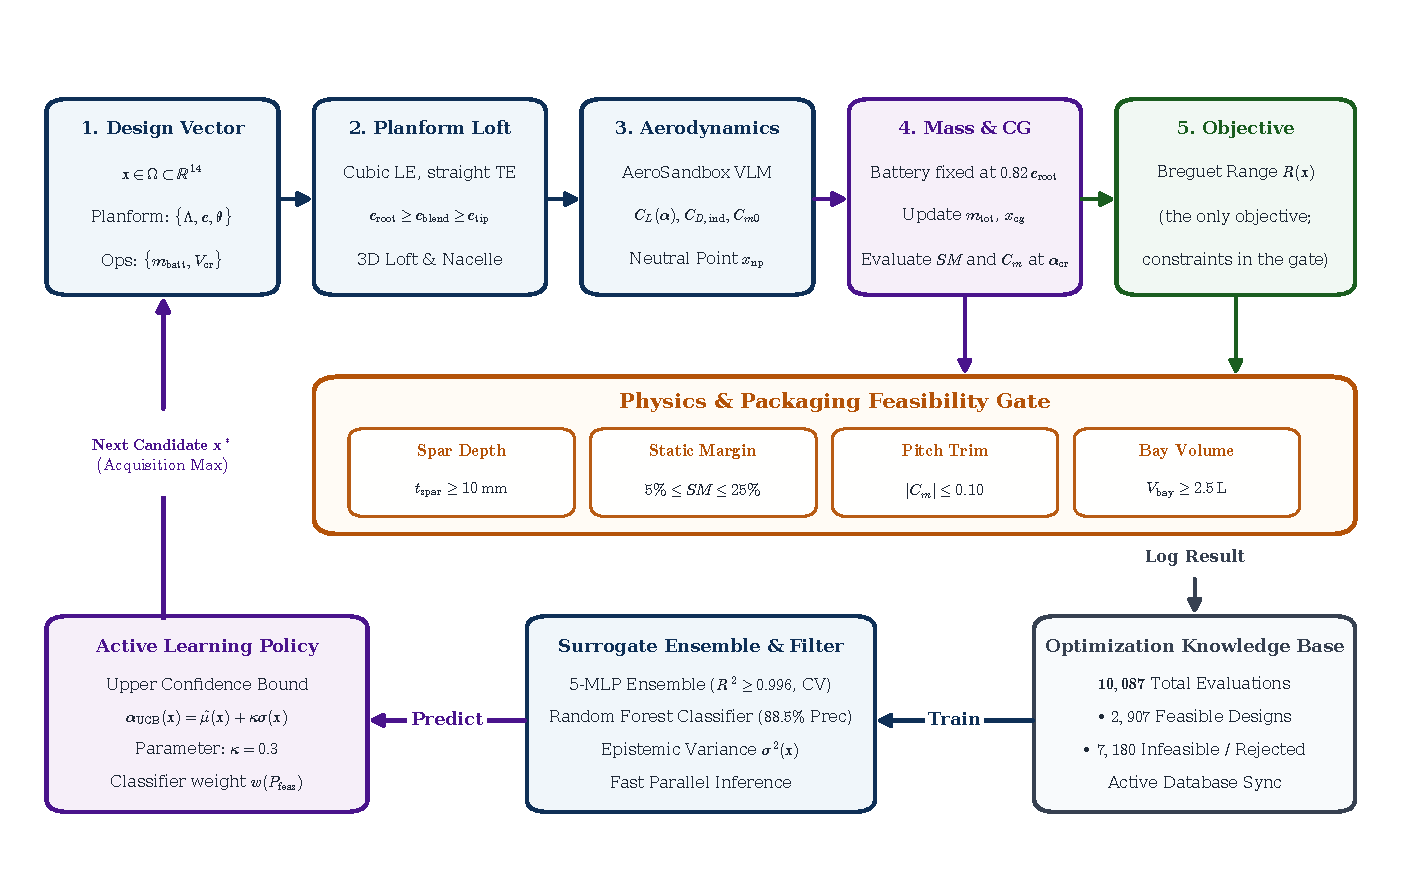
\includegraphics[width=0.92\linewidth]{figures/figure3_trim_loop_architecture.pdf}
\caption{Evaluation and search architecture. For every design vector the evaluator builds the clamped planform, runs the VLM, recomputes total mass and center of gravity with the battery centroid fixed at $0.82\,c_{r}$, and checks the static-margin, trim, spar-depth and bay-volume constraints. The classifier and surrogate ensemble then guide the active-learning acquisition. No battery position is solved for inside the loop.}
\label{fig:trim_loop_architecture}
\end{figure}

Every evaluation recomputes the total mass and center of gravity from the design vector (Fig.~\ref{fig:trim_loop_architecture}). The payload (at $0.20\,c_{r}$), avionics (at $0.25\,c_{r}$) and motor (at $c_{r} + 0.02\,\mathrm{m}$) are fixed point masses, the airframe mass $1.0 + 1.5\,S_{\mathrm{ref}}$\,kg acts at $0.40$ MAC behind the MAC leading edge, and the battery mass $m_{\mathrm{b}}$ is a design variable. The battery centroid is held fixed at $x_{\mathrm{batt}} = 0.82\,c_{r}$ ($f_{b} = 0.82$) for every design:
\begin{equation}
x_{\mathrm{cg}} = \frac{\sum_i m_i x_i + m_{\mathrm{b}}\, x_{\mathrm{batt}}}{m_{\mathrm{total}}}, \qquad x_{\mathrm{batt}} = 0.82\,c_{r}.
\end{equation}
The battery position is therefore an input to the optimization and not a quantity solved for: the evaluator contains no inversion for $x_{\mathrm{batt}}$. The static margin follows from the VLM-computed neutral point $x_{\mathrm{np}}$ and this center of gravity, $SM = (x_{\mathrm{np}} - x_{\mathrm{cg}})/\bar{c}$. A design is feasible only if $SM \in [0.05, 0.25]$ and $|C_m| \le 0.10$ at cruise (hard constraints), the center-body volume exceeds $2.5\,\mathrm{L}$ ($g_6$) and the spar depth is at least $10\,\mathrm{mm}$; a center of gravity outside $15$ to $40\%$ MAC is penalized softly. For the best design of the original campaign these constraints give natural pitch trim ($C_m = -0.019$) with $SM = 22.5\%$ and near-zero trim drag ($1.1\%$ of total drag). Table~\ref{tab:mass} shows how range and static margin change when the airframe mass model is scaled by $0.7$ and $1.3$, and Section~\ref{sec:robustness} reports the sensitivity of the best designs of all search arms to the battery position and mass.

A post-hoc inversion of the same moment balance is available for a single design, for example to ask which battery position would give a target static margin $SM^{\ast}$, with $x_{\mathrm{cg,target}} = x_{\mathrm{np}} - SM^{\ast}\bar{c}$:
\begin{equation}
x_{\mathrm{batt}} = \frac{m_{\mathrm{total}}\, x_{\mathrm{cg,target}} - \sum_i m_i x_i}{m_{\mathrm{b}}}.
\end{equation}
This inversion was applied after the optimization to the best design of the original campaign only. Fig.~\ref{fig:trim_sensitivity} is the corresponding post-hoc battery-position sweep and shows the feasible corridor around the chosen value of $0.82\,c_{r}$.

\begin{figure}[htbp]
\centering
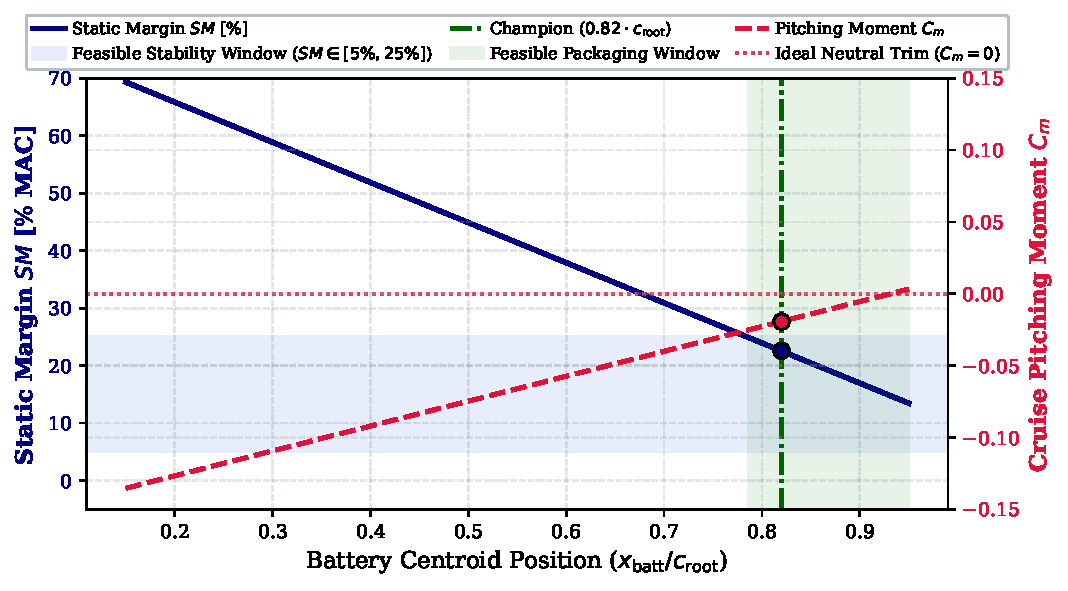
\includegraphics[width=0.95\linewidth]{figures/figure4_trim_sensitivity.pdf}
\caption{Post-hoc battery-position sweep on the original-campaign champion geometry: longitudinal trim and static stability as a function of battery centroid position ($x_{\mathrm{batt}} / c_{r}$), with all other mass moments held fixed. The feasible corridor ($SM \in [5\%, 25\%]$, $|C_m| \le 0.10$) spans $x_{\mathrm{batt}}/c_r$ from $0.79$ to $0.95$. The optimization fixes the battery at $0.82 \cdot c_{r}$ (green vertical line), which lies inside this corridor and gives $SM = 22.5\%$ and near-zero natural trim ($C_m = -0.019$).}
\label{fig:trim_sensitivity}
\end{figure}

